\newpage
\section{Array}
Una struttura dati molto conosciuta e chiamata array.
\begin{definition}[Array]
Gli array sono delle strutture dati omogenea, statiche e lineari implementate mediante un gruppo di celle contigue di memoria dello stesso tipo.
\end{definition}

Di seguito due esempi grafici di array uno di interi ed uno di stringhe, da notare sotto la posizione degli elementi nell'array che si conta partendo dallo 0.
\begin{figure}[h!]
    \centering
    \begin{subfigure}{.5\textwidth}
        \centering
        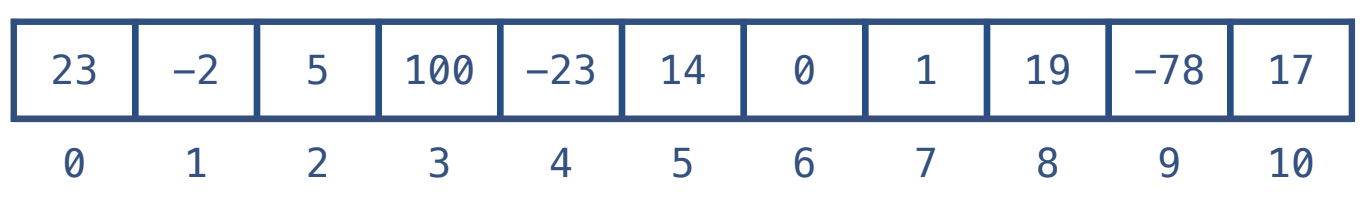
\includegraphics[width=9cm]{images/esempio-array-1.png}
        \caption{}
    \end{subfigure}
    \hfill
    \begin{subfigure}{.4\textwidth}
        \centering
        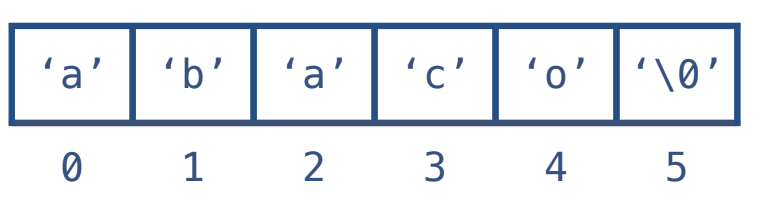
\includegraphics[width=6cm]{images/esempio-array-2.png}
        \caption{}
    \end{subfigure}
    \caption{In (a) un array lungo 11 di interi, in (b) un array lungo 6 di caratteri}
\end{figure}
\begin{note}
Nota che nell'array di caratteri sopra nell'ultima posizione c'è sempre $\setminus0$ (Null).
\end{note}
Negli array si accede mediante l'indice della posizione nella sequenza. Si possono inoltre effetturare sugli elementi tutte le operazioni definte sul tipo corrispondete agli elementi dell'array.
\begin{example}
Alcuni esempi di accesso ed operazioni su gli arrey sopra:
\begin{itemize}
    \item a[6] == 0 \hspace{.5cm} a[3] == 100 \hspace{.5cm} b[2] == 'a' 
    \item a[4] = a[5] + a[7] \: \: (a[5] == 14, a[7] == 1, quindi il risultato sarà 14 + 1 = 15)  
\end{itemize}
\end{example}

Inoltre possiamo dire che gli array sono allocati in memoria quando il controllo del flusso a tempo di esecuzione entra nel blocco in cui sono definiti e sono distrutti quando il controllo esce dal blocco.\\\\
Il nome dell'array è una variabile che contiene la locazione di memoria in cui è memorizzata la prima cella. Essendo che le celle sono contigue e hanno tutte lo stesso tipo basta infatti conoscere la posizione della prima cella per poi, tramite una semplice operazione algebrica di somma, accedere a quelle successive. In generale possiamo scrivere che:
\begin{center}
    $a[i] \: \: = \: \: \sigma(\rho(a) + size(type(a)) \times i)$
\end{center}
\begin{example}
Se abbiamo un array di lunghezza 11, ed chiamiamo la prima locazione (quella dove è contenuto il primo elemento dell'array) loc1, per raggiungere la posizione numero 10 basterà eseguire l'operazione loc1 + 32*10.
\end{example}
Questo consente l'accesso diretto agli elementi degli array con una sola operazione indipendentemente dalla lunghezza dell'array (consto di accesso costante). 

\subsection{BinarySearch}
\textbf{Problema:} Dato un elemento (o chiave) k, determinare se esiste all’interno di un array ordinato A di n elementi. Se l’elemento esiste, si restituisce la sua posizione, altrimenti -1. Soluzione con ricerca binaria.\\
\textbf{Proprietà:} $\forall i \in [0..n-1] \: . \: A[i] \leq A[i+1]$\\
Questa proprietà dice che l'array A deve essere obbligatoriamente ordinato, sennò la ricerca binaria non potrà esser fatta.
\begin{figure}[h!]
    \vspace{-10pt}
    \centering
    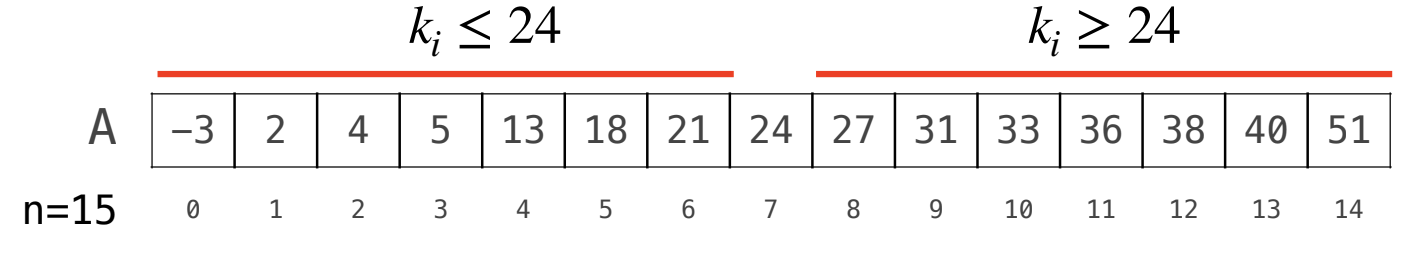
\includegraphics[width=9cm]{images/binary-search.png}
    \vspace{-8pt}
    \caption{Array A in BinarySearch}
    \label{fig:binary-search}
\end{figure}

\subsubsection{Codice dell'algoritmo}
\begin{lstlisting}[language=Javascript, caption=Codice BinarySearch]
function binSearch(k,A) {
    var pos:Int = -1;
    var sin:int = 0;
    var dx:Int = n - 1;
    while(sin <= dx && pos == -1){
        const cen:int = (sin + dx)/2;
        if (A[cen] == k) {pos = cen}
        else if (k < A[cen]) {dx = cen - 1}
        else {sin = cen + 1}
    }
    return pos;
}
\end{lstlisting}
Di seguito una spiegazione del funzionamento dell'algoritmo:
\begin{itemize}
    \item \textbf{Righe 2-4:} Andiamo ad inizializzare 3 variabili: "pos" che indicherà la posizione dell'elemento da cercare, viene inizializzata a -1 perché nel caso non si trovasse ritorna così -1. \\
    "Sin" che indica il capo sinistro della posizione che stiamo analizzando, e "dx" che indica il capo destro, sono entrambi inizialmente inizializzati come gli estremi dell'array.
    \item \textbf{Riga 5:} La condizione del while dice in sintesi che finché non abbiamo trovato il valore (pos == -1) e finchè "sin" e "dx" non si scambiano (che vorrebbe dire che abbiamo finito le iterazioni possibili), continuare a ciclare.
    \item \textbf{Righe 6-9:} All'interno del while quello che andiamo a fare e prendere il centro della porzione dell'array che stiamo considerando (inizialmente il centro dell'interno array) e vedere se il valore che dobbiamo cercare si trova in quella posizione, e in tal caso finiamo, è minore, e quindi si troverà alla sinistra del centro, o maggiore, in tal caso si troverà alla destra; nel caso non si sia trovato ci spostiamo ad analizzare la parte destra o sinistra asseconda del risultato. Eseguiamo questa operazioni finché è consentito dal ciclo.
\end{itemize}
\begin{note}
Nota che a noi non ci importa se la porzione è pari o dispari, quello che ci ritornerà esclude il resto.
\end{note}
\begin{example}
Esempio con l'array in figura \ref{fig:binary-search} cercando il valore 18.
\begin{table}[h!]
    \centering
    \setlength{\tabcolsep}{10pt}
    \renewcommand{\arraystretch}{1.8}
    \begin{tabular}{|c|c|c|c|c|}
    \hline
        pos & sin & dx & cen & A[cen]  \\\hline
        -1 & 0 & 14 & 7 & 24  \\\hline 
        -1 & 0 & 6 & 3 & 5  \\\hline
        -1 & 4 & 6 & 5 & \textbf{18}  \\
    \hline
    \end{tabular}
    \hspace{1cm}
    \begin{tabular}{|c|c|}
    \hline
        Iterazioni & Dimensione A \\\hline
        1 & n \: = \: n$/2^0$  \\\hline 
        2 & n/2 \: = \: n$/2^1$ \\\hline
        3 & n/4 \: = \: n$/2^2$ \\\hline
        ... & ... \\
    \hline
    \end{tabular}
    \caption{Esempio di funzionamento dell'algoritmo a sinistra e numero iterazione a destra}
\end{table}
\end{example}

\subsubsection{Calcolo caso pessimo e migliore}
Per calcolare il caso pessimo partiamo guardando la tabella sopra, notiamo che in questo algoritmo verranno eseguite $n/2^i$ operazioni, quindi il massimo possibile dipende da quanto è grande $i$. Per andare a trovare $i$ basta:
\begin{center}
    $n/2^i = 1$ \hspace{.3cm} $n = 2^i$ \hspace{.3cm} $\log_2n = \log_22^i$ \hspace{.3cm} $i = \log_2n \in O(\log_n)$
\end{center}
Questo caso è o quando k si trova agli estremi o quando k non c'è nell'array, e quindi ritorna -1.